\documentclass{article}

\usepackage{siunitx} % Provides the \SI{}{} and \si{} command for typesetting SI units
\usepackage{graphicx} % Required for the inclusion of images
\usepackage{amsmath} % Required for some math elements 
\usepackage[export]{adjustbox} % loads also graphicx
\usepackage{listings}
\usepackage{matlab-prettifier}
\usepackage{float}

\usepackage{titlesec}
\usepackage{caption}
\usepackage{subcaption}

\newcommand{\R}{\mathbb{R}}

\usepackage{xcolor}

\DeclareCaptionFont{white}{\color{white}}
\DeclareCaptionFormat{listing}{%
  \parbox{\textwidth}{\colorbox{gray}{\parbox{\textwidth}{#1#2#3}}\vskip-4pt}}
\captionsetup[lstlisting]{format=listing,labelfont=white,textfont=white}
\lstset{frame=lrb,xleftmargin=\fboxsep,xrightmargin=-\fboxsep}
\titleformat{\section}[runin]
  {\normalfont\Large\bfseries}{\thesection}{1em}{}
\titleformat{\subsection}[runin]
  {\normalfont\large\bfseries}{\thesubsection}{1em}{}


\setlength\parindent{0pt} % Removes all indentation from paragraphs

\renewcommand{\labelenumi}{\alph{enumi}.} % Make numbering in the enumerate environment by letter rather than number (e.g. section 6)

%\usepackage{times} % Uncomment to use the Times New Roman font

%----------------------------------------------------------------------------------------
%	DOCUMENT INFORMATION
%----------------------------------------------------------------------------------------

\title{AMATH 353: Homework 6 \\Due April, 20 2018 \\ ID: 1064712} % Title

\author{Trent \textsc{Yarosevich}} % Author name

\date{\today} % Date for the report

\begin{document}
\maketitle % Insert the title, author and date
\setlength\parindent{1cm}

\begin{center}
\begin{tabular}{l r}
%Date Performed: December 1, 2017 \\ % Date the experiment was performed
Instructor: Jeremy Upsal % Instructor/supervisor
\end{tabular}
\end{center}

% If you wish to include an abstract, uncomment the lines below
% \begin{abstract}
% Abstract text
% \end{abstract}

%----------------------------------------------------------------------------------------
%	SECTION 1
%----------------------------------------------------------------------------------------
\section*{Part 1.)} 
With $u(x,0) = \sin(x)$ and $u_t(x,0) = xe^{-x^2}$ and $c = 1$ we arrive at the following using the D'Alembert solution:
\begin{equation}
\begin{aligned}
\int_{x-ct}^{x+ct} xe^{-x^2} = \frac{1}{2}e^{-(x-ct)^2} - \frac{1}{2}e^{-(x+ct)^2}\\
\\
\text{Then plugging this into the solution we get }\\
\\
u(x,t) = \frac{1}{2}(\sin (x - t) + \sin (x + t)) +  \frac{1}{4}e^{-(x-ct)^2} - \frac{1}{4}e^{-(x+ct)^2}\\
\end{aligned}
\end{equation}
This problem relates to the previous two insofar as the solution is composed of the sum of four traveling waves, two of which appear in 8.4, and the other two in 8.5. For me personally, the easiest way to visualize this is to consider the solutions from 8.4 and 8.5 independently, and to rewrite the solution from 8.4 as follows:
\begin{equation}
u(x,t) = \cos (t)\sin (x)
\end{equation}
And then 8.5:
\begin{equation}
\frac{1}{4}e^{-(x-t)^2} - \frac{1}{4}e^{-(x+t)^2}
\end{equation}
Equation (2) is a sin wave with amplitude varying over time from -1 to 1, and equation (3) is composed of two traveling wave pulses. The solution in equation (1) above is the sum of these, so there is a sin wave with varying amplitude over time, and two wave pulses are travelling 'through' this wave so to speak. Thus the solution in (3) will behave just like equation (1) except at those regions where it is being disrupted by the two wave pulses. The following figures show the initial sin wave with no disruption from the wave pulses (which are 0 for all x at $t=0$) and three $t$ values that show how it disrupts the wave.

\begin{figure}[H]
  \centering
  \begin{minipage}[b]{0.49\textwidth}
    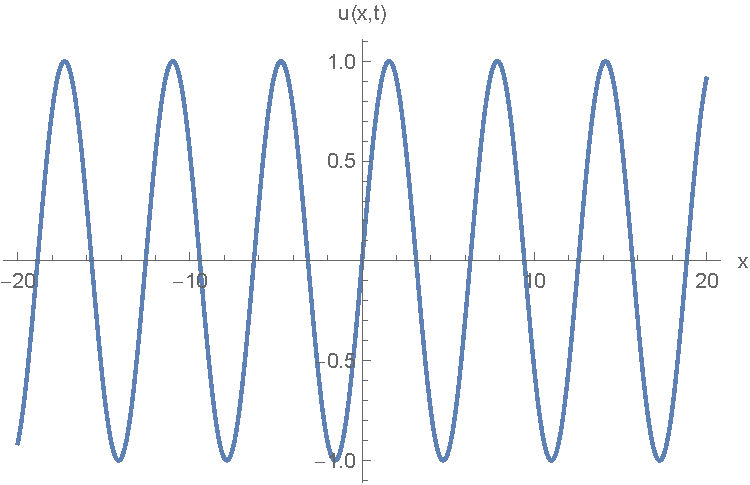
\includegraphics[width=\textwidth]{plot_t_0.pdf}
    \caption{$t = 0$}

  \end{minipage}
  \hfill
  \begin{minipage}[b]{0.49\textwidth}
    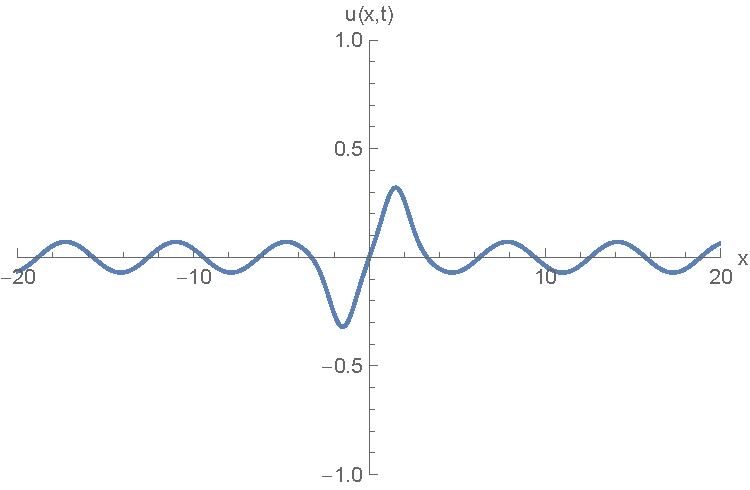
\includegraphics[width=\textwidth]{plot_t_15.pdf}
    \caption{$t = 1.5$}

  \end{minipage}
    \hfill
  \begin{minipage}[b]{0.49\textwidth}
    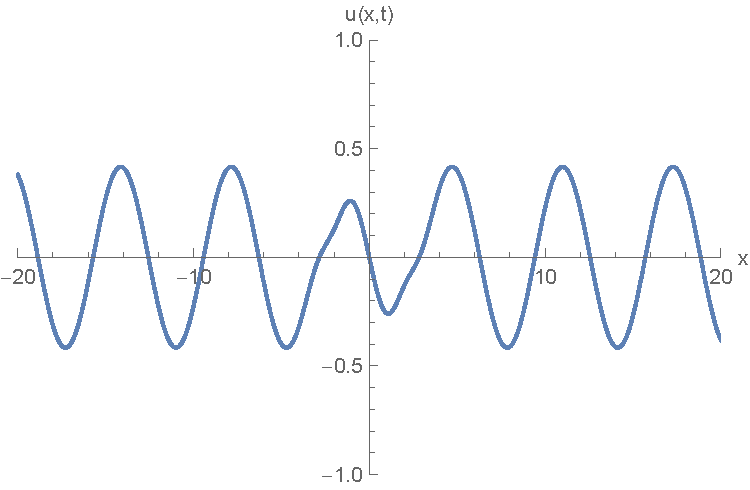
\includegraphics[width=\textwidth]{plot_t_2.pdf}
    \caption{$t = 2$}

  \end{minipage}
    \hfill
  \begin{minipage}[b]{0.49\textwidth}
    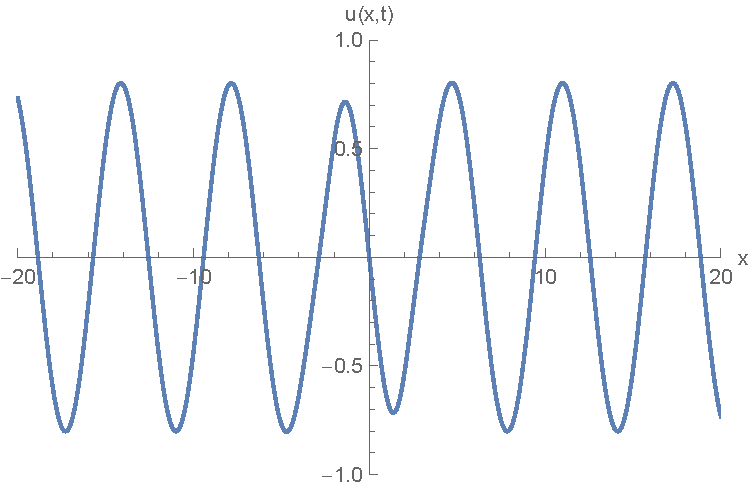
\includegraphics[width=\textwidth]{plot_t_25.pdf}
    \caption{$t = 2.5$}

  \end{minipage}
\end{figure}
A few observations can be made. In figure 2, we see the varying amplitude of the sin wave is very small, making the disruptions from the wave pulses more obvious than in figure 4, for example. Furthermore we can observe in figures 2 and 3 that the left-moving wave pulse has a negative value, and the right-moving a positive one, thus we can see that the left moving wave pulse disrupts the sin wave by 'pulling' it down, and the right-moving pulse does the opposite.
\section*{Part 2.)}
From the D'Alembert solution we get:
\begin{equation}
\begin{aligned}
u(x,t) = \frac{1}{2} ( (x - 2t) + (x + 2t)) + \frac{1}{8} \int_{x-2t}^{x+2t} y^2dy\\
u(x,t) = \frac{1}{2} ( (x - 2t) + (x + 2t)) + \frac{1}{8} \int_{x-2t}^{x+2t} y^2dy\\
u(x,t) = \frac{1}{2} ( (x - 2t) + (x + 2t)) + \frac{1}{8}(\frac{1}{3}(x+2t)^3 - \frac{1}{3}(x-2t)^3)
\end{aligned}
\end{equation}
The resulting solution is the sum of two unbounded lines moving in opposite directions, the sum of which is both algebraically and geometrically pretty obvious, that is $u(x, t) = x$ (note I am only talking about $f(x-2t) + f(x+2t)$). The definite integral of $u_t$ contributes two opposite polynomials moving in opposite directions. The resulting solution is unbounded as $x \to \pm \inf$. Presumably this is not a useful solution for modeling real phenomenon as the solution blows up pretty quickly.
\end{document}